\chapter{A térképgenerálás módja}
\label{chap:tervezes}

Mivel korábban már több játékot is készítettem ami négyzetrács alapú térképet használ, most szerettem volna megismerni, hogy a hexagon alapú térképek, hogyan készülnek, ezért választottam a hexagont a programom térképének alapjául a szakdolgozatomban. Ehhez \textit{eltolásos koordináta-rendszer}t fogok használni a megjelenítésben és a tárolásban, mivel téglalap alakú térképet szeretnék használni és ehhez a megoldáshoz a fentebb említettek alapján ez tünt célszerű döntésnek. Mivel az \textit{eltolásos koordináta-rendszer}ben a számítások bonyolultabbak, mint a többi ismertetett koordináta-rendszerben, ezért a számításokhoz a koordinátákat átalakítom a \textit{kocka koordináta-rendszer}beli megfelelőjére és azzal fogom elvégezni a számításokat, majd pedig visszaalakítom a tároláshoz és a megjelenítéshez. Az útkereső algoritmusok közül az \textit{A*}-algoritmusra esett a választásom, mivel általános esetben ez bizonyult hatékonynak.

\section{Stílus és modellek}

A játékban szereplő grafikai stílusként a low-poly irányzatot választottam. Ehhez kezdetben saját készítésű modelleket használtam. Mivel a térkép generálásához nagy meny\-nyi\-sé\-gű, kidolgozott, egységes kinézetű modell szükséges, és a dolgozat tárgyköre elsődlegesen nem grafikai modellezés, ezért az Interneten kerestem további modelleket.

A játék fejlesztése során három dimenziós modelleket használtam, mert ezáltal lehetőség nyílt arra, hogy a térképet forgatni lehessen és különböző szemszögekből meg lehessen azt nézni. Úgy ítéltem meg, hogy ez több előnnyel jár, mint amennyi plusz energiát követel meg.

A térkép hexagonokból épül fel, és a hexagonháló egyik fő jellemzője az, hogy a háló szélein lévő hexagonok nem egy vonalba esnek. Ennek az előnyeit és hátrányait korábban \aref{sec:hexagon} fejezetben már taglaltam. Jelen esetben a már említett problémák nem jelentkeznek, mivel nem kell igazodni semmilyen körülhatároló objektumhoz.

A generálás során a térképen a különböző környezeti viszonyoknak megfelelően más és más objektumok jelennek meg. \Aref{tab:models}. táblázatban azt láthatjuk, hogy a különböző objektum tipusokból a különböző környezeti viszonyok között mennyi áll rendelkezésre.

\begin{figure}[h!]
  \centering
  \begin{tabular}{ | c | c | c | c | }
    \hline
     & Sivatag & Normál & Havas \\ \hline
    Kisebb növények / kövek & 14 & 6 & 0 \\ \hline
    Fák & 4 & 4 & 4 \\ \hline
    Épületek & 6 & 6 & 6 \\ \hline
    Hegyek & 2 & 2 & 2 \\ \hline
  \end{tabular}
  \caption{A különböző típusokhoz és környezeti viszonyokhoz tartozó objektumok száma.}
  \label{tab:models}
\end{figure}
 \newpage
\section{Kamera}

A programban izometrikus megjelenítési módot használok. Ez a megoldás gyakori a stratégiai játékoknál. A legtöbb számítógépes játék esetében az izometrikus nézet nem fedi teljes mértékben a matematikai értelemben vett izometrikus nézetet. A számítógépes játékokban eleinte azért alkalmazták az izometriát, mivel ezt egyszerűbb volt megjeleníteni a korabeli hardvereken. Manapság  izometrikusnak nevezik (matematikai értelemben helytelenül) azokat az eseteket, amikor a kamera tengelye tipikusan 30, 45, 53 vagy 60 fokos szöget zár be a játék térképének síkjával. (Ezek közül talán a legérdekesebb az 53 fok, ami a régebbi kijelzőknek a felbontásának arányából (4:3) adódott.)

A 45 és a 60 fokos megoldás nyújtotta azt a hatást amit szerettem volna elérni, végül a 45 fokos szög mellett döntöttem. Ehhez 60 fokos látószöget (FOV, \textit{Field of View}) alkalmaztam. A kamera körbeforgatható a horizontális tengely körül 360 fokban, ezt a 3D-s modellek miatt van lehetőség megoldani, ezáltal a térkép objektumainak elhelyezkedése szemléletesebb. Lehetőség van arra, hogy a térképre ráközelítsünk vagy távolodjunk tőle, ennek megvan a felső és alsó határa. Igyekeztem úgy megválasztani ezeket a határokat, hogy ne lehessen túl közel, vagy túl távol vinni a kamerát a térképtől. A kamera természetesen a térkép mentén mozgatható mind a 4 irányban. 

A játékfejlesztésben az egyik legnehezebb feladat a kamera kezelés megvalósítása, mivel ha jól működik senki sem veszi észre, ha pedig hibásan működik akkor a teljes felhasználói élményt tönkreteheti. Ezért úgy döntöttem, hogy egy olyan kódot használok fel a Unity store-ból amit már korábban is használtam és kisebb módosítások alkalmazásával minden szempontot megvalósít \cite{RTS_Camera}.

\section{Generálás lépései}

Bemenetként a térkép fő jellemzőit, a generált térképpel szembeni elvárásokat kapja paraméterezésként a program. Bizonyos paraméterek szabályozhatóak a generálás után is (mint például a hőmérséklet), de a többségük nem.

A térképnek a főbb paraméterei szabályozhatóak: méret, környezeti viszonyok, domborzat, folyók, növényzet, épületek. Egyéb apró paraméterei nem módosíthatóak a játék használata közben, de a Unity szerkesztőben (\textit{Unity editor}) az Inspector ablakokban a többségük állítható. Ezt azért alakítottam így ki mert nem akartam a felhasználói felületet túl komplikálttá tenni, inkább az egyszerűségre törekedtem. Az Inspector ablakon lehetséges módosítani a poligonhálókat, textúrákat, árnyalókat, skalár paramétereket.

A térkép egy többlépcsős folyamat eredményeként készül el. Ezeket a lépéseket a következő pontokban fogom bemutatni.
\begin{itemize}
\item Első lépésként szükségünk lesz egy csempére (tile), ami az alapelem lesz a térképen. Erre a célra én egy 3D-s hexagon modellt használtam különböző textúrákkal. A különböző textúrák és a modellek csak a Unity-n belül egy úgynevezett Inspector panelen módosíthatóak. A játékban jelenleg a hexagonhoz 6 különböző textúra szerepel (fű, homok, hó, víz, jég, óceán (térkép széle)).
\item Ezen kívül szükség van a generálni kívánt térkép méreteire (szélesség, magasság). Ezek a paraméterek a generálás előtt a felhasználó által is szabályozhatóak bizonyos intervallumon.
\end{itemize}

\subsection{Térkép széleinek létrehozása}

A térkép körülhatárolására egy speciális hexagon textúrát hoztam létre, ami az óceánt szimbolizálja. Ez gyakori megközelítés a stratégiai játékok esetén a térkép körülhatárolására (például \textit{Civilization IV: Colonization}). A játékfejlesztők különböző módszerekkel határolják körbe a térképet, mint például felhők, hegyek, várfalak, óceánok. Ennek a célja, hogy a karakterek ne tudjanak a széleket határoló néhány mezőre lépni.

A beállított magasság és szélesség értékeken felül fog az algoritmus minden egyes szélre egy plusz sort/oszlopot generálni. Amikor a felhasználó a térkép bejárható részének méreteit $x \times y$ -nak adta meg, a kapott térkép mérete $(x+2) \times (y+2)$ méretű lesz.

\subsection{Domborzat kialakítása}

A második elem ami majd a térképen meghatározásra kerül, az a domborzat. Ez két fajta magasságban jelenik meg (domb, hegy), amihez két különböző modellt használok. A térkép méreteihez viszonyítva lehet majd százalékos arányban kifejezni a domborzat mennyiséget, egy $0\%$-tól $40\%$-ig terjedő skálán. Ezt az intervallumot találtam megfelelőnek ahhoz, hogy ha sok hegyet akarunk akkor sok hegyet kapjunk, de még a karakterek által bejárható maradhasson a térkép. Ezt az intervallumot a generálás előtt a felhasználó be tudja állítani. A hegyek és a dombok véletlenszerű pozícióban helyezkednek el. A különböző környezeti viszonyokhoz három különböző textúra áll rendelkezésre (fű, homok, hó). A hegyek és a dombok egyenletes eloszlás szerint kerülnek a térkép egyes részeire. Ha egy olyan mezőt választott ki az algoritmus amin már volt egy hegy/domb, akkor újrakezdi a keresést.

\subsection{Folyók elhelyezése}

A folyók generálásakor két különböző esetet különböztettem meg; amikor vannak hegyek és amikor nincsenek. Amikor vannak hegyek akkor az egyik hegy lábától egy másik vizes mezőig (a térkép szélei vagy egy már meglévő folyó) generál az algoritmus folyót az útkereső algoritmus felhasználásával. Abban az esetben, amikor nincs egy darab hegy sem, akkor az algoritmus vagy véletlenszerűen választ egy mezőt a térképen és egy vizes mezőig generál. A domborzathoz hasonlóan a vizes mezők mértéke is szabályozható a felhasználó által a generálás előtt. Ez is a domborzatnál már megismert $0\%$-tól $40\%$-ig tartó skálán mozog a térkép méretéhez viszonyítva. A környezeti viszonyokhoz alkalmazkodva kétfajta textúra jöhet szóba, úgy mint a normál és a jeges. Ez a módszer viszonylag könnyen implementálható az útkereső algoritmus ismeretében, és kellően egyedi megjelenést tud kölcsönözni a térképnek. Keletkezhetnek szigetek (\ref{fig:Island}. ábra), szélesebb folyók, torkolatok (\ref{fig:Branch}. ábra). Ezen kívül minden vizes mező hozzáadódik egy listához aminek majd a vízszint meghatározásában lesz szerepe.

\begin{figure}[h!]
\centering
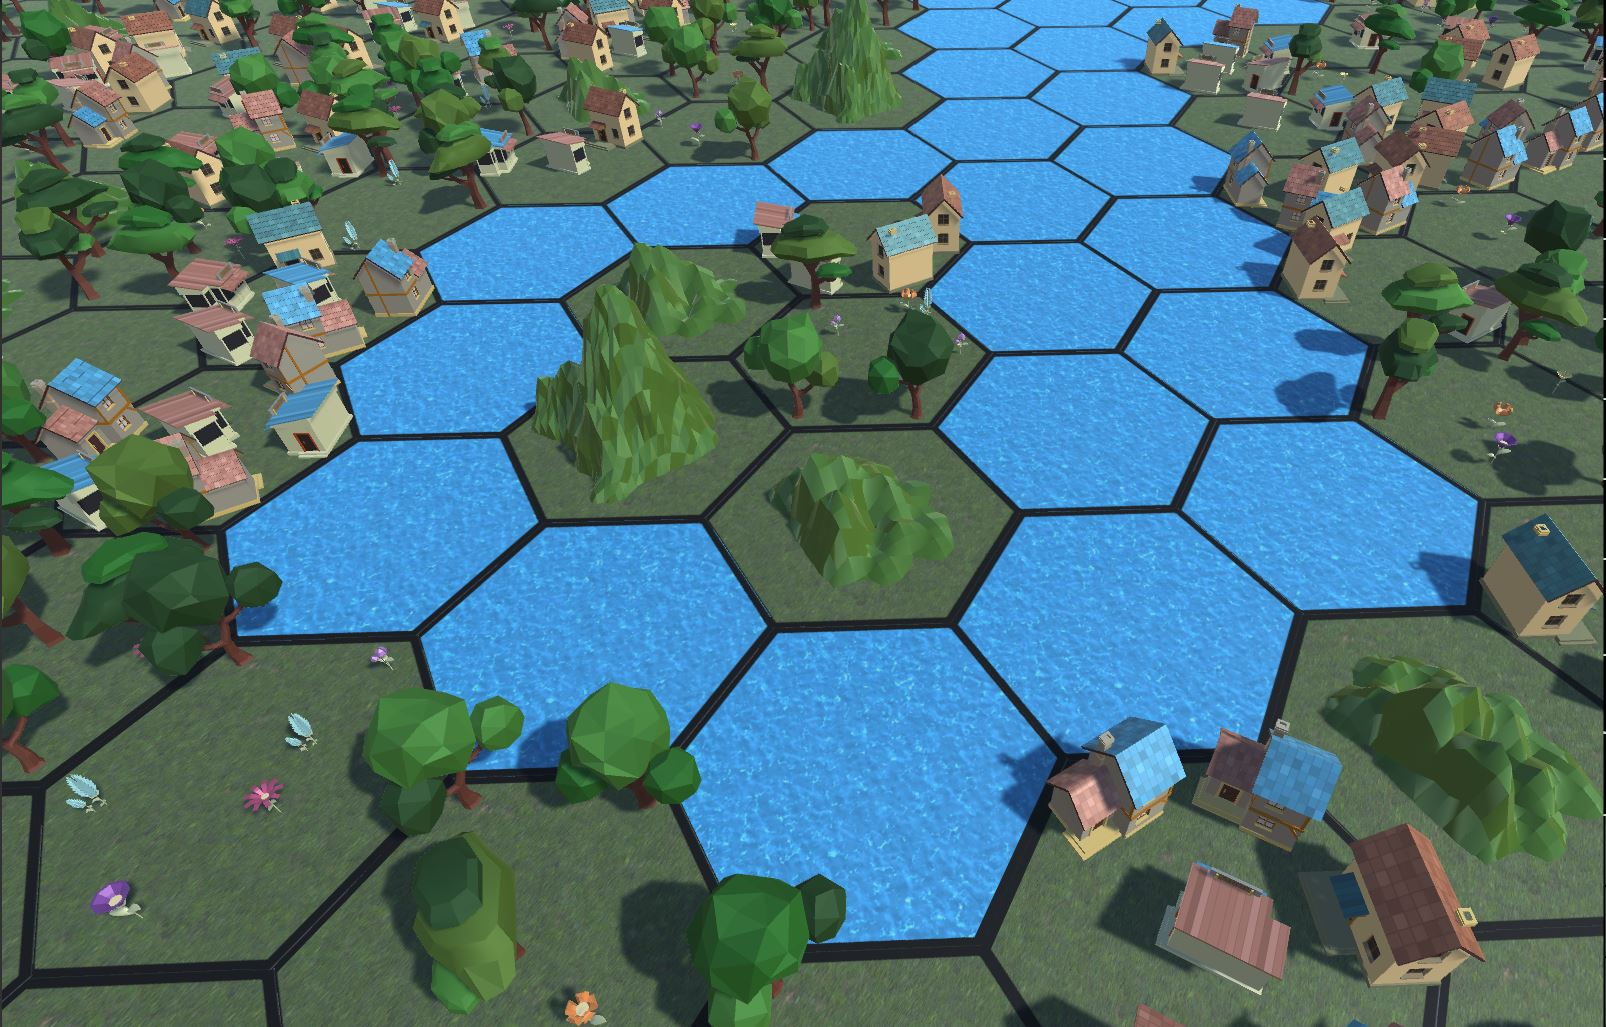
\includegraphics[scale=0.3]{kepek/Island.JPG}
\caption{Sziget}
\label{fig:Island}
\end{figure}

\begin{figure}[h!]
\centering
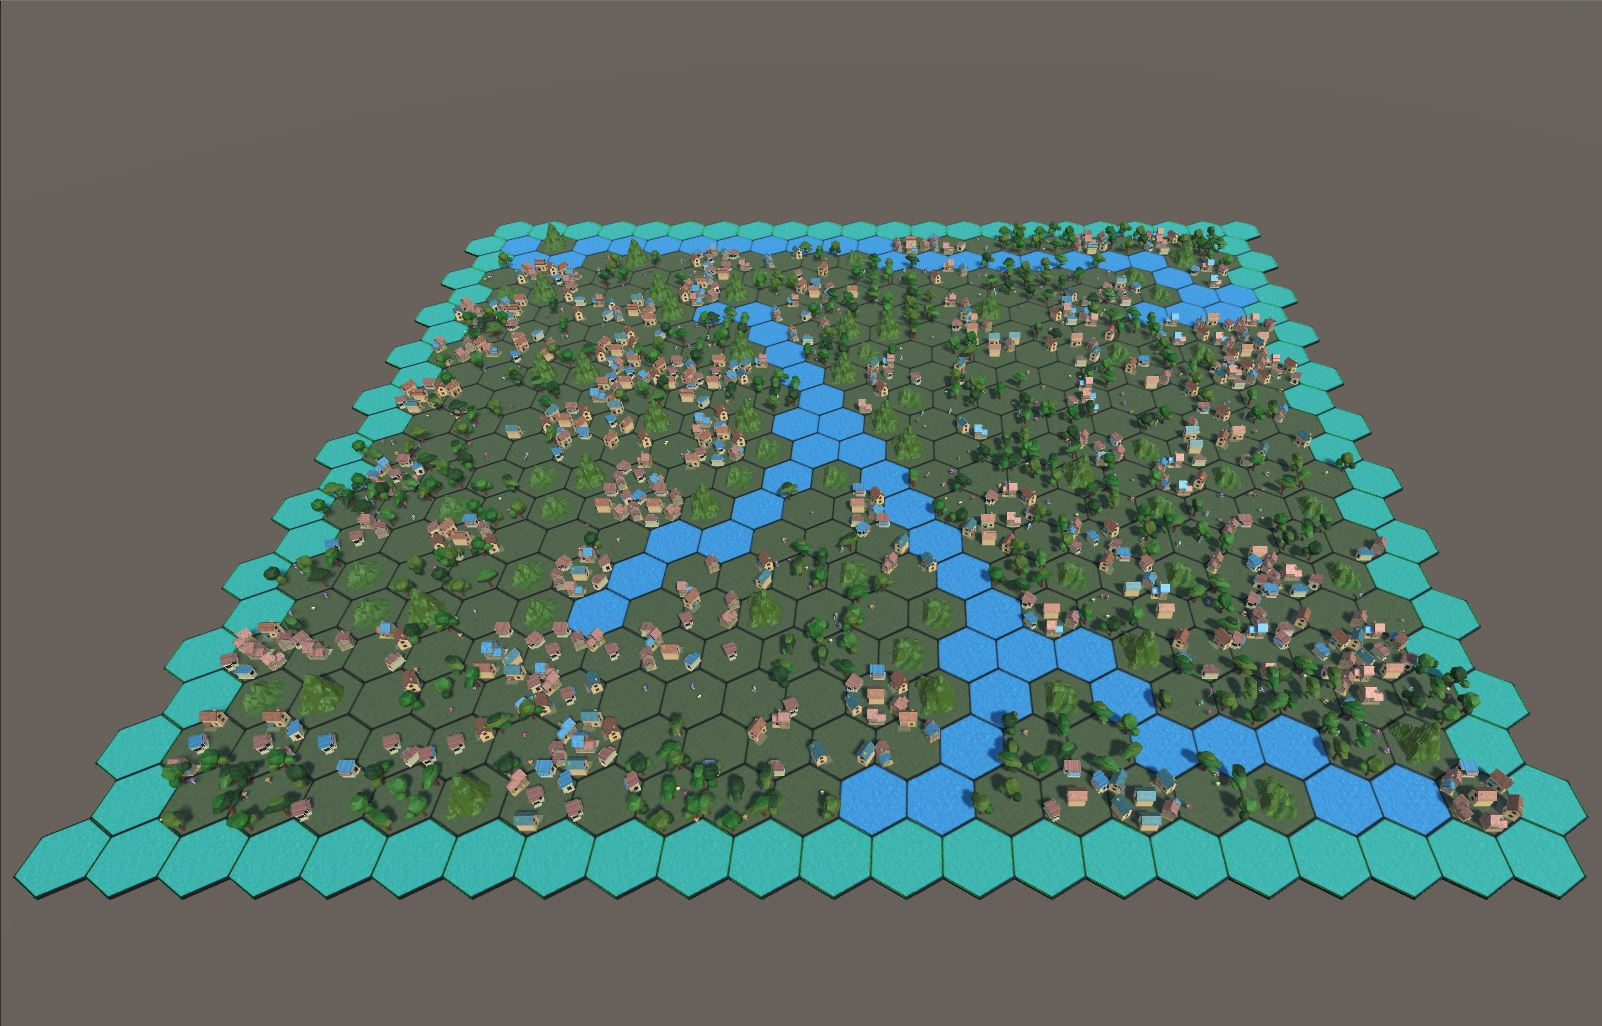
\includegraphics[scale=0.3]{kepek/Branch.JPG}
\caption{Elágazások a folyón}
\label{fig:Branch}
\end{figure}

\subsection{Sík területek generálása}

Az algoritmus minden olyan mezőre, ahová még nem generált domborzatot vagy folyót, oda sík terültet fog generálni. Ezek sima hexagonokból fognak állni és a további paraméterek segítségével kerülhetnek majd rá épületek, fák, virágok. Itt is a már megszokott 3 textúra áll majd rendelkezésre, úgy mint fű, homok és jég stílusú.

\subsection{Vízszint meghatározása}

A vízszint meghatározása minden mezőre a növényzet generálásához szükséges. A vízszint a vizes mezőktől távolodva lineárisan csökken. Ezáltal megvalósítható, hogy minél távolabb van egy mező a víztől, annál kisebb az esélye, hogy sok növényzet legyen rajta. A hőmérséklet mellett még a vízszint fog közrejátszani abban, hogy hogyan ,,száradjanak ki'' a különböző mezők.

\subsection{Épületek elhelyezése}

Úgy terveztem, hogy az épületek és a fák 7 fix pozícióban állhatnak a hexagonon (\ref{fig:Places}. ábra). Azért döntöttem a 7 fix pont mellett mert így egyszerűbb az algoritmus, mint ha véletlenszerű pozíciókban szerepelnének a hexagonon. Így nem kell vizsgálni, hogy az objektumok amiket elhelyezne az algoritmus azok ütköznek-e valamilyen egyéb objektummal a térképen. Mindössze csak arra kell figyelni, hogy egy helyen csak egy objektumot tudjunk elhelyezni. A további fejlesztések esetén például az úthálózatot is könnyebben megvalósíthatónak tartom mintha véletlenszerű helyeken lennének és nem is feltétlenül lenne jobb megoldás. Kétfajta épület van. A házak esetén a környezeti változások a falakat nem, csak a háztetők textúráját érintik. Így például havas stílusú hexagonon az épület teteje is havas lesz (\ref{fig:Buildings}. ábra).

\begin{figure}[h!]
\centering
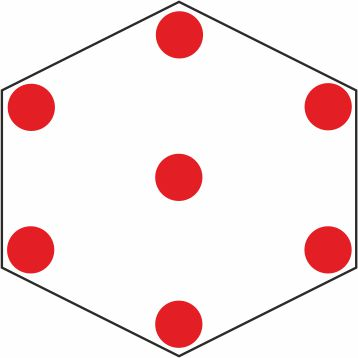
\includegraphics[scale=1]{kepek/Places.jpg}
\caption{Az épületek és fák elhelyezkedési pontjai a hexagonon}
\label{fig:Places}
\end{figure}

\begin{figure}[h!]
\centering
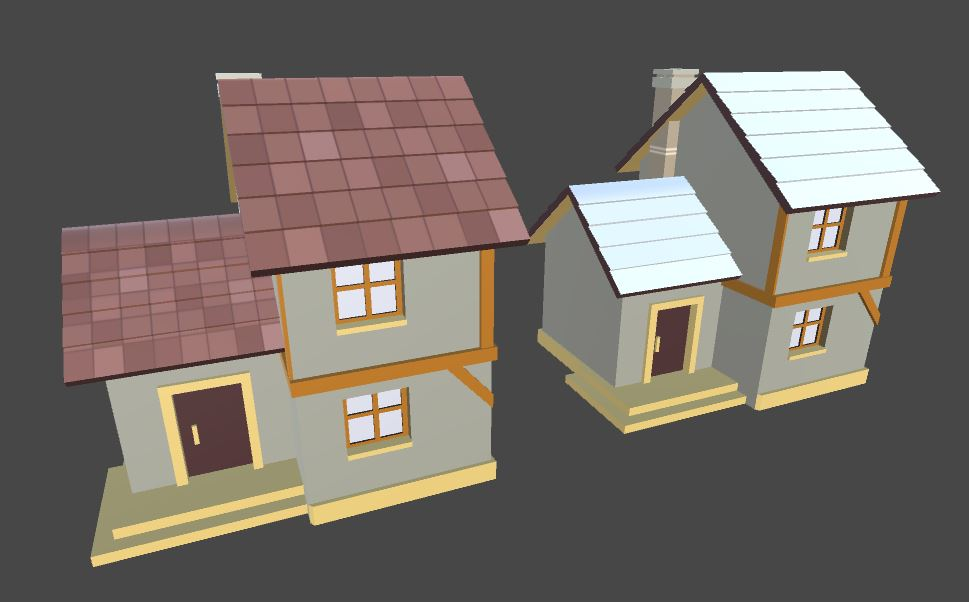
\includegraphics[scale=0.3]{kepek/Buildings.JPG}
\caption[épület]{Egy épület normál körülmények között (bal oldal) és havas körülmények között (jobb oldal). \footnotemark}
\label{fig:Buildings}
\end{figure}

\footnotetext{www.assetstore.unity3d.com/en/\#!/content/50095}

\subsection{Növényzet kialakítása}

A növényzetet úgy tervezem megvalósítani, hogy két csoportra bontom azt. Az egyikbe a fák, a másikba pedig a kisebb objektumok, például virágok, kaktuszok, kövek kerültek. Mind a két csoportot másképpen valósítottam meg.

\subsubsection{Fák elhelyezése}

Az épületeknél már megismert módszerrel 7 fix helyre kerülhetnek egy mezőn belül. Két különböző modell fog szerepelni a játékban az időjárási viszonyoknak megfelelően pedig három különböző módon jelenhetnek majd meg. A különböző viszonyoknak megfelelően fog különböző szinekből generálni a fáknak lomb színt az algoritmus (\ref{fig:Tree_Normal}., \ref{fig:Tree_Fall}. és \ref{fig:Tree_Winter}. ábrák), ezt egy listán lehet majd megadni a különböző esetekhez. A fák csak sík mezőkön generálódhatnak majd, ezáltal egyszerűsítve a generálást.

\begin{figure}[h!]
\centering
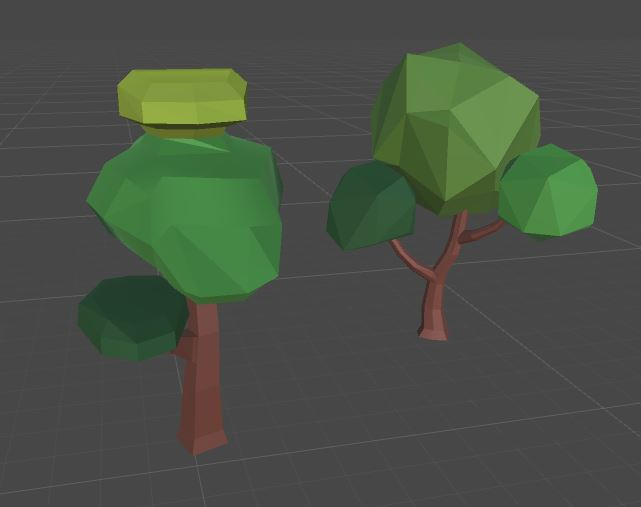
\includegraphics[scale=0.32]{kepek/Tree_Normal.JPG}
\caption[normal]{Normál esetben a fák lombja a zöld különböző árnyalataiból állhat. \footnotemark}
\label{fig:Tree_Normal}
\end{figure}

\footnotetext{www.assetstore.unity3d.com/en/\#!/content/52217}

\begin{figure}[h!]
\centering
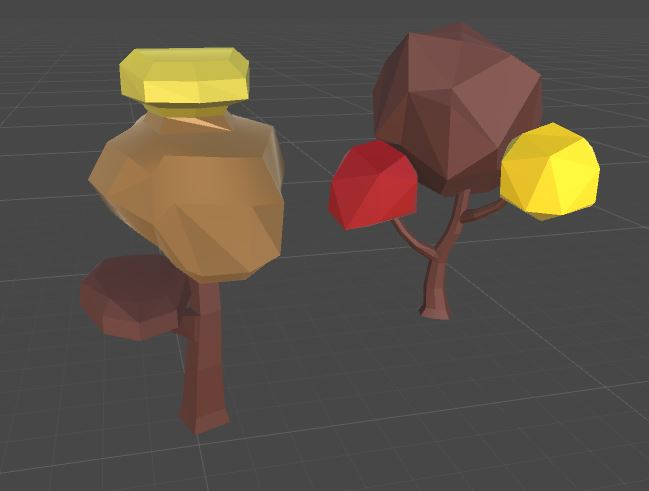
\includegraphics[scale=0.32]{kepek/Tree_Fall.JPG}
\caption[Ősz]{“Ősz” A lomb színei ebben az esetben több különböző szín árnyalatából tevődik össze (piros, barna, sárga). \footnotemark}
\label{fig:Tree_Fall}
\end{figure}

\footnotetext{www.assetstore.unity3d.com/en/\#!/content/52217}

\begin{figure}[h!]
\centering
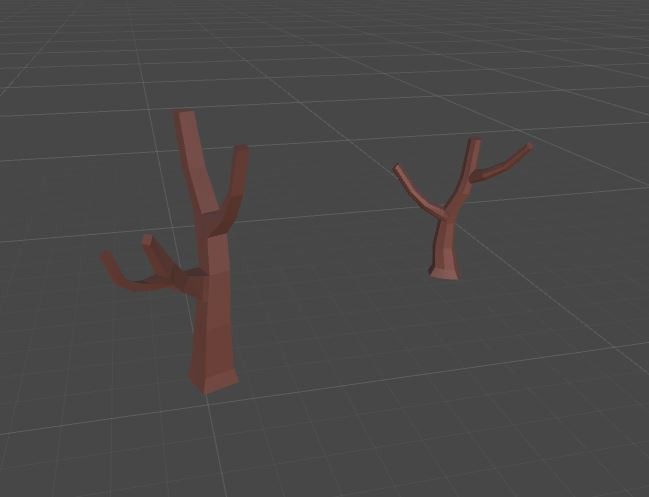
\includegraphics[scale=0.32]{kepek/Tree_Winter.JPG}
\caption[tél]{Kiszáradt vagy jeges esetben az algoritmus elrejti a lombokat. \footnotemark}
\label{fig:Tree_Winter}
\end{figure}

\footnotetext{www.assetstore.unity3d.com/en/\#!/content/52217}

\newpage
\subsubsection{Kisebb objektumok elhelyezése}

Véletlenszerű pozíciókban generálja az algoritmus a sík mezőkön. A kisebb objektumok közé tartoznak a virágok, kaktuszok, kövek (\ref{fig:Flowers}. és \ref{fig:Cactus}. ábrák). A kaktuszok és a kövek a homokos területeken, míg a virágok a füves területeken fordulnak elő. 

\begin{figure}[h!]
\centering
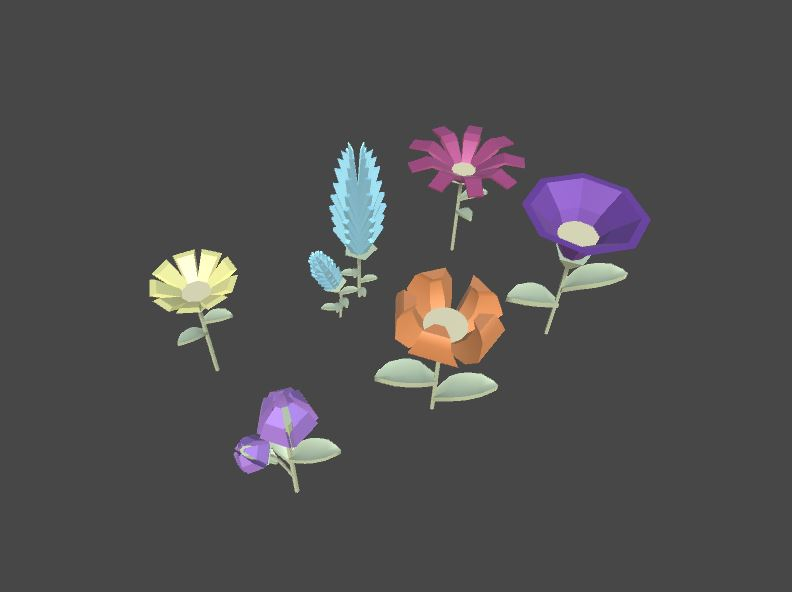
\includegraphics[scale=0.4]{kepek/Flowers.JPG}
\caption[Virágok]{Virágok \footnotemark}
\label{fig:Flowers}
\end{figure}

\footnotetext{www.assetstore.unity3d.com/en/\#!/content/47083}

\begin{figure}[h!]
\centering
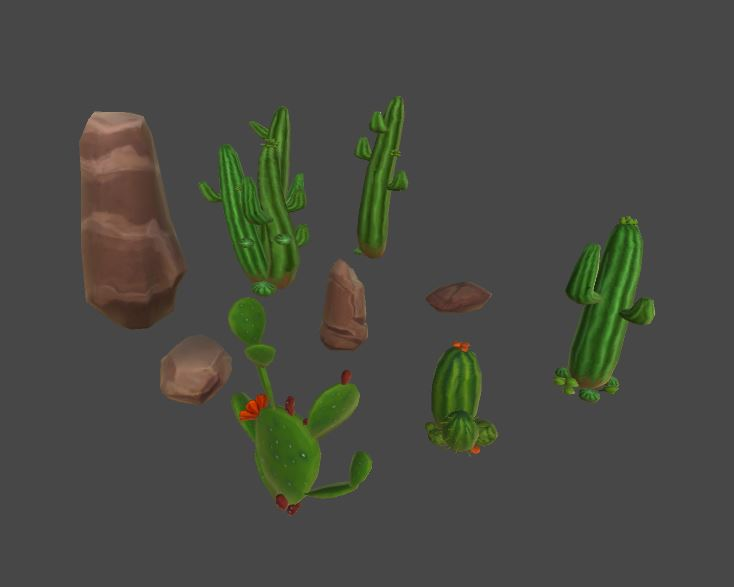
\includegraphics[scale=0.4]{kepek/Cactus.JPG}
\caption[Kaktuszok és kövek]{Kaktuszok és kövek \footnotemark} 
\label{fig:Cactus}
\end{figure}

\footnotetext{www.assetstore.unity3d.com/en/\#!/content/11547}

\subsection{Hőmérséklet beállítása}

Lehetőség van az évszakok között váltogatni. Ez a funkció fontos a játék tovább fejlesztésével kapcsolatban, mivel a játékban szerepet kap majd az évszakok változása. A tavasz és az ősz nem változtatja az alap hőmérsékleti viszonyokat csak a nyár és a tél módosítja a globális hőmérsékletet egy konstans értékkel. 

A különböző objektumokra a térképen elfoglalt helyük alapján és egyéb tulajdonságaik miatt különböző módon hat majd az időjárás. Ezt mutatom be a következőkben lépésről-lépésre.

Elsődlegesen egy globális hőmérséklet paramétert készítek, ami minden egyes mezőre egységes mértékben vonatkozik és a többi paraméter pedig ehhez adódik hozzá. Ezzel már lehet a különböző ,,évszakokat'' tesztelni a játékban.

Ekkor az algoritmus a térkép felső és alsó része között egy átmenetet valósít meg, mint ha egy nagyobb kontinens lenne. Ennek a paraméternek lehetséges negatív és pozitív értéket is megadni, amelyek azt befolyásolják, hogy milyen mértékben fog növekedni vagy csökkenni a hőmérséklet mezőről mezőre.

\begin{figure}[h!]
\centering
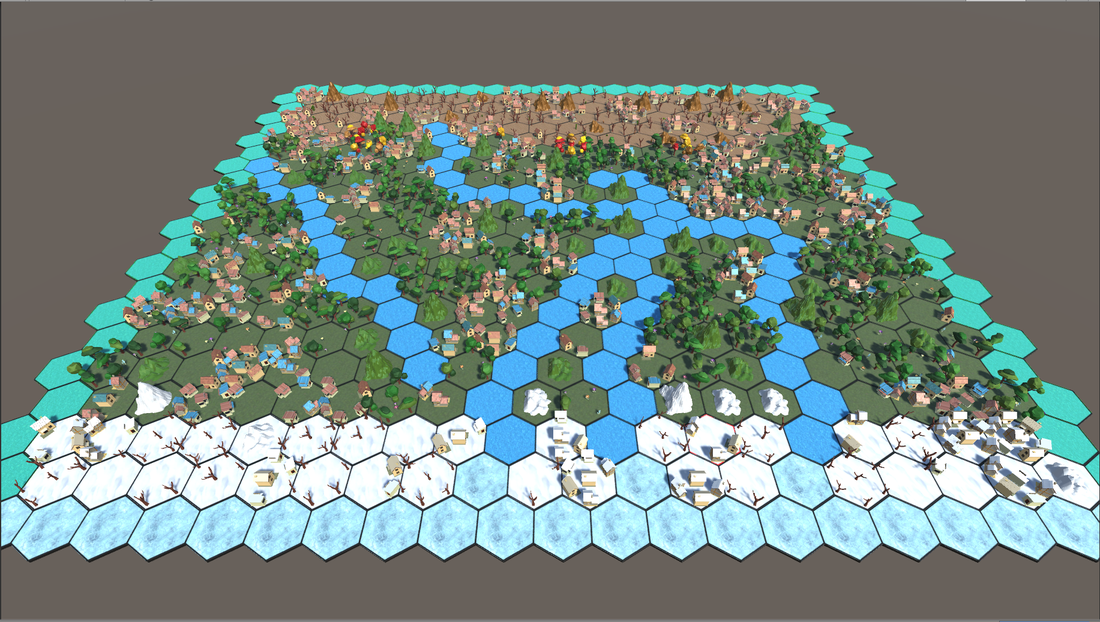
\includegraphics[scale=0.5]{kepek/transition.png}
\caption{Hőmérséklet átmenet}
\label{fig:transition}
\end{figure}

Ezt követően egy külön paraméterrel dinamikusan lehet a generált térképen változtatni a hőmérsékletet. Ez is változtatható pozitív és negatív értékűre annak függvényében, hogy melegebb vagy hidegebb környezetet szeretnénk elérni.

Végezetül a különböző objektumok tulajdonságai közé tartozik, hogy a hőmérsékletre és annak változására hogyan reagálnak. Ez alatt azt értem, hogy a vizes mezők alacsonyabb hőmérséklet mellett kezdenek el befagyni, mint a sík mezők vagy azok a mezők hamarabb kezdenek el kiszáradni, ahol kevesebb a víz.

\Aref{fig:transition} ábrán láthatjuk a hőmérséklet és hőmérséklet átmenet alkalmazásának eredményét.
